\chapter{The Optical Flow Equation}
\sectionmark{The Optical Flow Equation}
\section{The Brightness constancy assumption}
The optical flow equation is derived from what is called brightness constancy assumption of Horn and Schunck \cite{HS}. Let $\textbf{r}(t) = (x(t),y(t))$ be the parametrization of some line in $\Omega$ and let 
\begin{align*}
\frac{d \textbf{r}}{dt} = \textbf{w}(\textbf{r}(t),t) = \left[ u(\textbf{r}(t),t),v(\textbf{r}(t),t) \right]^T
\end{align*}
be the flow vector along this line. The brightness constancy assumption says that a point moving with velocity $\textbf{w}(\xi(t),t)$ along the trajectory $\textbf{r}(t)$ over time $t$ does not change its appearance. This means that if the scene has the same lighting, then movement of an object along a trajectory does not change its brightness. In mathematical notation this is (under perfect conditions) equivalent to the following:
\begin{align*}
\frac{d}{dt}f(\textbf{r}(t),t) = 0.
\end{align*}
By using the chain rule for differentiation one gets
\begin{align*}
\frac{\partial f}{\partial x} u + \frac{\partial f}{\partial y} v + \frac{\partial f}{\partial t} = 0,
\end{align*}
or equivalently
\begin{align}
\nabla f^T  \textbf{w} + f_t = 0.
\end{align}
Unfortunately, since the flow consists of 2 components, this equation is not enough to determine the flow, but only the component of the flow in the direction of the gradient, or what is known as the normal flow. This is called the Aperture problem and it is illustrated in Figure (\ref{ApertureProblem}). Thus another constraint 

\begin{figure}
    \centering
    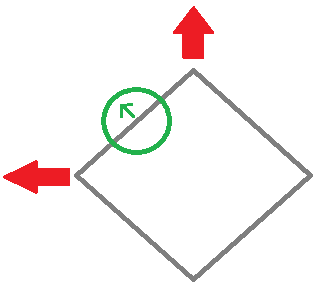
\includegraphics[scale=0.5]{Figures/ApertureProblem.png}
    \caption{Illustration of the Aperture problem. Moving the gray rectangle in the direction of any of the two red arrows both give the movement shown by the green arrow if seen through the green circled aperture.}
    \label{ApertureProblem}
\end{figure}



Let now
\begin{align*}
\rho(\textbf{w}) = \nabla f \cdot \textbf{w} + f_t
\end{align*}
To minimize $\rho$, Horn and Schunck used a quadratic penalizer, which is equivalent to least-squares minimization. Least-squares minimization is very sensitive to outliers. In the case of the data term, these outliers would be noise in the image (a pixel that jumps from low intensity to high intensity without corresponding to the motion of an object). Due to the poor robustness to outliers of least-squares minimization other penalization functions have been suggested. Black and Anandan \cite{Black199675} proposed several subquadratic penalizer functions, arguing that a subquadratic penalizer would improve the robustness in the presence of outliers.
and assuming the data term has some quadratic dependence on $\rho$, one can define
\begin{align}
\label{DataPenalize}
M(u,v) = \Psi_M(\rho^2),
\end{align}
where $\Psi_M$ is some penalizing function aiming to minimize $\rho$. 
\section{The Aperture Problem}
Since the flow consists of 2 components, the brightness constancy assumption alone is not enough to determine the flow, but only the components of the flow in the direction of the gradient, or what is known as the normal flow. This is called the Aperture problem, and to be able to compute the components of the flow vector one needs another constraint. This other constraint is known as the smoothness constraint.